\documentclass{beamer}

\usepackage[utf8]{inputenc}
\usepackage[T1]{fontenc}
\usepackage[french]{babel}
\usepackage[babel=true]{csquotes}
\frenchbsetup{StandardLists=true}
\usepackage{graphicx}
\usepackage{color}
\usepackage{hyperref}
\usepackage{float}
\usepackage{pifont}
\usepackage{enumitem}
\hypersetup{colorlinks,linkcolor=,urlcolor=blue}

\mode<presentation>
{
%\usetheme{Bergen}
%\usetheme{Boadilla}
\usetheme{Madrid}
%\usetheme{AnnArbor}
%\usetheme{CambridgeUS}
%\usetheme{EastLansing}
%\usetheme{Rochester}
%\usetheme{Montpellier}
%\usetheme{Berkeley}

\setbeamercovered{transparent}
}

\title[Dev. Mobiles]{Présentation d'un projet de développement d'application mobile :\\LotoQuinote}
\author{David~Boisedu et Alexandre~Boyer}
\institute[]{L3 Informatique}
\date{\today}


\AtBeginSection[]
{
  \begin{frame}
  %\frametitle{Sommaire}
  %\tableofcontents[currentsection, hideothersubsections, pausesubsections]
  \vfill
  \centering
  \begin{beamercolorbox}[sep=8pt,center,shadow=true,rounded=true]{title}
    \usebeamerfont{title}\insertsectionhead\par%
  \end{beamercolorbox}
  \vfill
  \end{frame} 
}

\setbeamersize{text margin left=1cm, text margin right=1cm}


\begin{document}
\logo{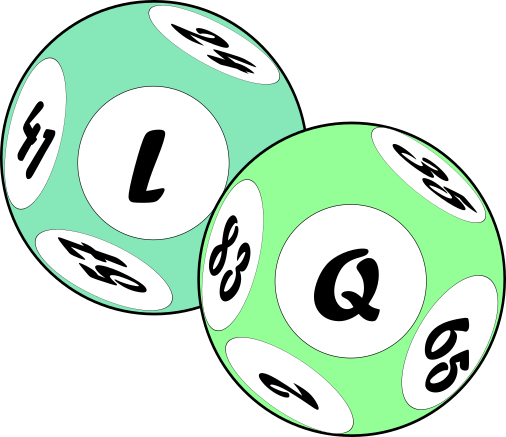
\includegraphics[height=5mm]{Images/logo.png}}

\begin{frame}
    \titlepage
\end{frame}

\section{Introduction}

\begin{frame}{Introduction}
    \begin{center}
        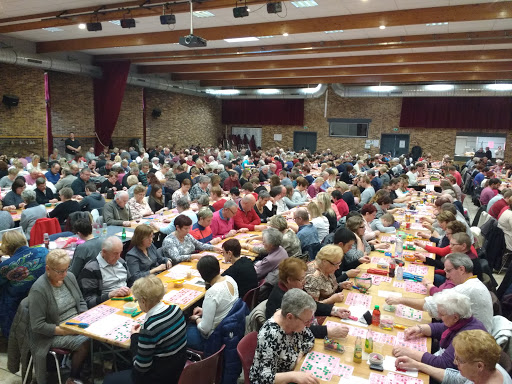
\includegraphics[height=5cm]{Images/lotoquine_evenement.jpg}
    \end{center}
    \begin{center}
        Le loto-quine : une passion
    \end{center}
\end{frame}

\begin{frame}{Introduction}
    \begin{center}
        Principe du jeu
    \end{center}
    \begin{center}
        \begin{semiverbatim}
            Chaque joueur est muni d’un carton de loto et de pions. Parmi 90 boules numérotées, un numéro est tiré au sort et le joueur place son pion sur le numéro sorti s’il est \newline mentionné sur son carton. Une fois son carton rempli, le joueur gagne le lot mis en jeu.
        \end{semiverbatim}
    \end{center}
\end{frame}

\begin{frame}{Introduction}
    \begin{columns}[T]
     \begin{column}[c]{5cm}
        \begin{center}
\includegraphics[height=3cm]{Images/loto_icon.png}
        \end{center}
     \end{column}
     \begin{column}[c]{5cm}
          \begin{center}
\includegraphics[height=3cm]{Images/note_icon.png}
          \end{center}
     \end{column}
     \end{columns}
\end{frame}


\section{Présentation et objectif du projet}

\begin{frame}{Présentation et objectif du projet}
    \begin{columns}[T]
     \begin{column}[c]{5cm}
     Développer une application de suivi de tirage d'un loto-quine sous Android.
     \end{column}
     \begin{column}[c]{5cm}
          \begin{center}\includegraphics[height=3cm]{Images/cartons-français-de-jeu-de-loto-24190649.png} \end{center}
     \end{column}
     \end{columns}
\end{frame}

\begin{frame}{Présentation et objectifs du projet}

Doit permettre à l'utilisateur de :
\vspace{2em}
\begin{itemize}[label=\textbullet, font=\large \color{blue}]
    \item Créer un suivi de tirage
    \item Entrer les numéros du tirage dans ce suivi
    \item Consulter la liste complète du suivi de tirage
    \item Sauvegarder les numéros ajoutés à la liste
\end{itemize}
\end{frame}

\section{Choix technique}

\begin{frame}{Choix technique}
    \begin{columns}[T]
     \begin{column}[c]{5cm}
        \textbf{\LARGE{Android}}
        \vspace{3em}
        \newline Pourquoi choisir ce système d'exploitation ?
     \end{column}
     \begin{column}[c]{5cm}
          \begin{center}
\includegraphics[height=5cm]{Images/872px-Android_robot.svg.png} \end{center}
     \end{column}
     \end{columns}
    
\end{frame}

\begin{frame}{Choix technique}
    \begin{center}
        \fbox{\Large{Android Studio}}
    \end{center}
    \begin{center}
        Facilité de développement
    \end{center}
    \vspace{3em}
    \begin{center}
        \fbox{\Large{78,8\%}}
    \end{center}
    \begin{center}
        La part du marché des systèmes d'exploitation mobile (Q1 2020)
    \end{center}
\end{frame}

\section{Réalisation}

\begin{frame}{Réalisation}
    \begin{columns}[T]
    \begin{column}[c]{5cm}
        \textbf{Environnement logiciel}
        \vspace{2em}
        \begin{itemize}[label=\textbullet]
            \item Android Studio 
\includegraphics[height=0.5cm]{Images/1200px-Android_Studio_icon.svg.png}
            \item GitHub 
\includegraphics[height=0.5cm]{Images/1200px-Octicons-mark-github.svg.png}
            \item Inkscape 
\includegraphics[height=0.5cm]{Images/1200px-Inkscape_Logo.svg.png}
        \end{itemize}
    \end{column}
    \begin{column}[c]{5cm}
        \textbf{Autre plateformes utiles à la réalisation du projet}
        \vspace{1em}
        \begin{itemize}[label=\textbullet]
            \item Moqups.com 
\includegraphics[height=0.5cm]{Images/moqups.png}
            \item Trello 
\includegraphics[height=0.5cm]{Images/logo_trello.png}
            \item Messenger 
\includegraphics[height=0.5cm]{Images/1200px-Facebook_Messenger_4_Logo.svg.png}
        \end{itemize}
    \end{column}
    \end{columns}
\end{frame}

\section{Description générale de l'application}

\begin{frame}{Description générale de l'application}
    \begin{columns}[T] % contents are top vertically aligned
     \begin{column}[c]{5cm} % each column can also be its own environment
     La vue d'accueil
     \end{column}
     \begin{column}[c]{5cm} % alternative top-align that's better for graphics
          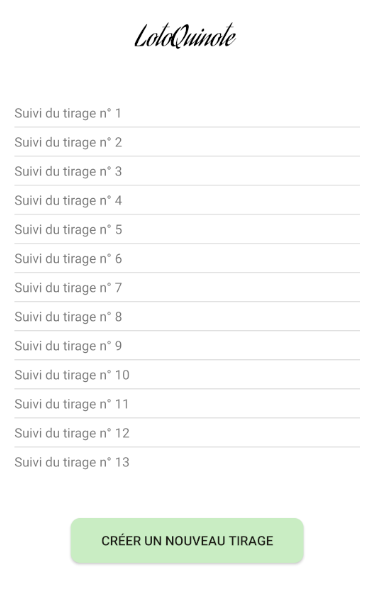
\includegraphics[height=8cm]{Images/accueil.png}
     \end{column}
     \end{columns}
\end{frame}

\begin{frame}{Description générale de l'application}
    \begin{columns}[T]
    \begin{column}[c]{5cm}
        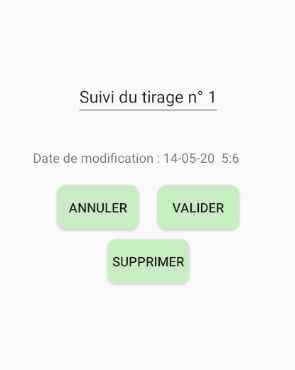
\includegraphics[height=6cm]{Images/edition.png}
    \end{column}
    \begin{column}[c]{5cm}
    La fonction d'édition
    \end{column}
    \end{columns}
\end{frame}

\begin{frame}{Description générale de l'application}
    \begin{columns}[T]
     \begin{column}[c]{5cm}
     La vue de suivi de tirage
     \end{column}
     \begin{column}[c]{5cm}
          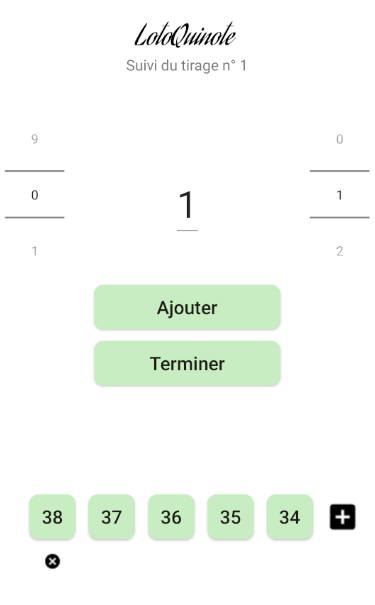
\includegraphics[height=8cm]{Images/suivi.png}
     \end{column}
     \end{columns}
\end{frame}

\begin{frame}{Description générale de l'application}
    \begin{columns}[T]
    \begin{column}[c]{5cm}
        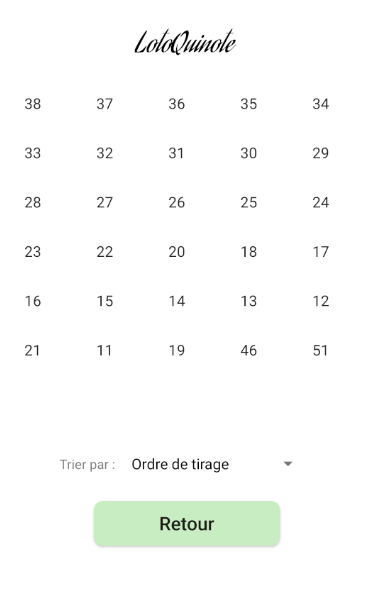
\includegraphics[height=6cm]{Images/liste.png}
    \end{column}
    \begin{column}[c]{5cm}
    La vue de la liste des numéros tirés
    \end{column}
    \end{columns}
\end{frame}

\section{Démonstration}

\section{Conclusion}

\begin{frame}{Conclusion}
    \begin{columns}[T]
    \begin{column}[c]{6cm}
        \textbf{Objectif atteint}
        \begin{itemize}[label=\ding{51}]
            \item Application de suivi de tirage
            \item Consigne respectée
        \end{itemize}
        \vspace{3em}
        \textbf{Nouvelles connaissances}
        \begin{itemize}[label=\ding{51}]
            \item Développement Android
            \item Git et GitHub
        \end{itemize}
    \end{column}
    \begin{column}[c]{6cm}
        \textbf{Travail en équipe}
        \begin{itemize}[label=\ding{51}]
            \item Organisation du travail
            \item Bonne coopération
        \end{itemize}
        \vspace{3em}
        \textbf{Améliorations possibles}
        \begin{itemize}[label=\ding{220}]
            \item Personnalisation de l'interface
            \item Gestion des joueurs/gains
        \end{itemize}
    \end{column}
    \end{columns}
\end{frame}

\begin{frame}{Conclusion}
    \begin{columns}[T]
    \begin{column}[c]{5cm}
        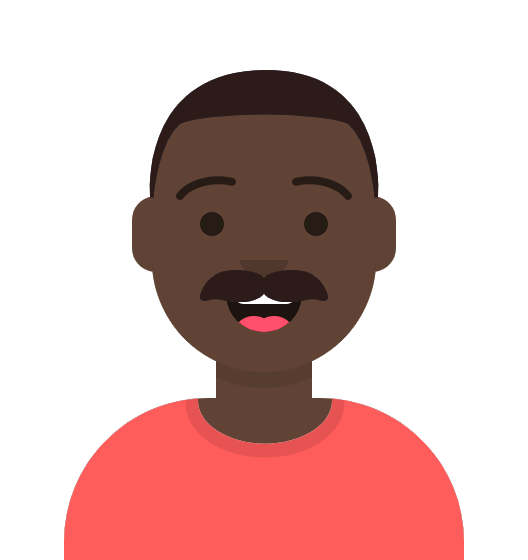
\includegraphics[height=5cm]{Images/avatar_david.png}
    \end{column}
    \begin{column}[c]{5cm}
        
\includegraphics[height=5cm]{Images/avatar_alexandre.png}
    \end{column}
    \end{columns}
    \begin{center}Merci beaucoup de votre attention !\end{center}
\end{frame}

\end{document}